% Generated by LitigCharts.PublicationFigures. Captions and provenance are sidecars.
\documentclass[10pt,tikz,border=5pt]{standalone}
\usepackage{lmodern}
\usetikzlibrary{patterns,patterns.meta}
\begin{document}
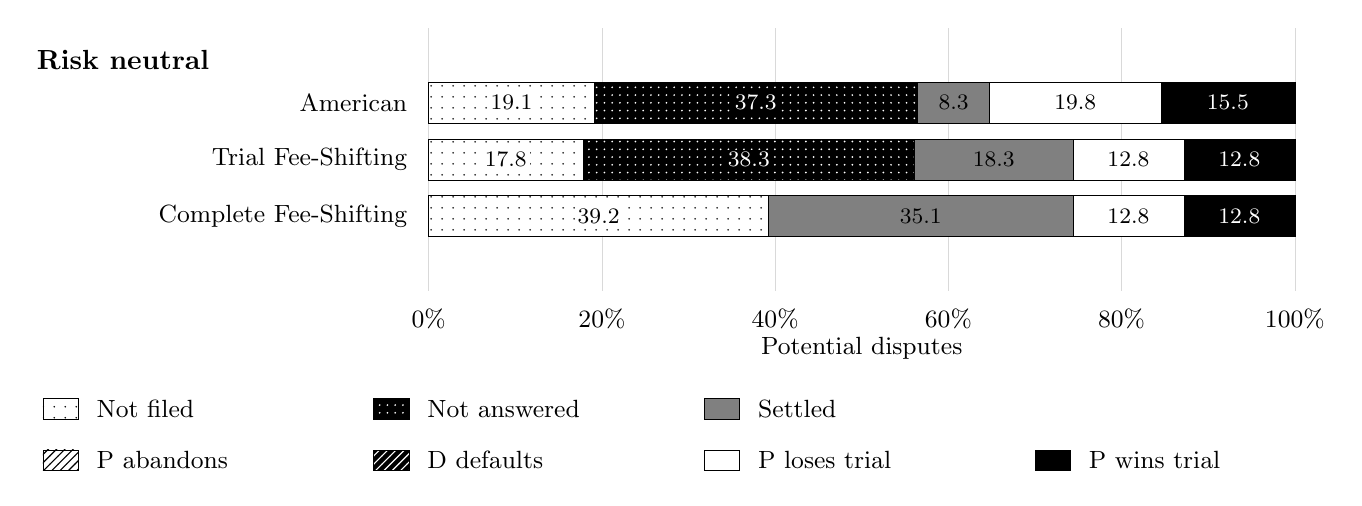
\begin{tikzpicture}[font=\small]\draw[black!15,line width=.2pt] (5.1,.65) -- (5.1,3.99);
\node[anchor=north] at (5.1,.55) {0\%};
\draw[black!15,line width=.2pt] (7.3,.65) -- (7.3,3.99);
\node[anchor=north] at (7.3,.55) {20\%};
\draw[black!15,line width=.2pt] (9.5,.65) -- (9.5,3.99);
\node[anchor=north] at (9.5,.55) {40\%};
\draw[black!15,line width=.2pt] (11.7,.65) -- (11.7,3.99);
\node[anchor=north] at (11.7,.55) {60\%};
\draw[black!15,line width=.2pt] (13.9,.65) -- (13.9,3.99);
\node[anchor=north] at (13.9,.55) {80\%};
\draw[black!15,line width=.2pt] (16.1,.65) -- (16.1,3.99);
\node[anchor=north] at (16.1,.55) {100\%};
\node[anchor=west,font=\bfseries] at (0,3.59) {\mbox{Risk} \mbox{neutral}};
\node[anchor=east] at (4.95,3.04) {American};
\path[preaction={fill=white,draw=none},pattern={Dots[distance=4pt,radius=.35pt]},pattern color=black,draw=black,line width=.25pt] (5.1,2.78) rectangle (7.201583,3.3);
\node[text=black,fill=white,font=\footnotesize,inner sep=1pt] at (6.150792,3.04) {19.1};
\path[preaction={fill=black,draw=none},pattern={Dots[distance=2.8pt,radius=.35pt]},pattern color=white,draw=black,line width=.25pt] (7.201583,2.78) rectangle (11.306552,3.3);
\node[text=white,fill=black,font=\footnotesize,inner sep=1pt] at (9.254068,3.04) {37.3};
\path[fill=black!50,draw=black,line width=.25pt] (11.306552,2.78) rectangle (12.224401,3.3);
\node[text=black,fill=none,font=\footnotesize,inner sep=1pt] at (11.765476,3.04) {8.3};
\path[fill=white,draw=black,line width=.25pt] (12.224401,2.78) rectangle (14.399101,3.3);
\node[text=black,fill=none,font=\footnotesize,inner sep=1pt] at (13.311751,3.04) {19.8};
\path[fill=black,draw=black,line width=.25pt] (14.399101,2.78) rectangle (16.099998,3.3);
\node[text=white,fill=none,font=\footnotesize,inner sep=1pt] at (15.249549,3.04) {15.5};
\node[anchor=east] at (4.95,2.32) {Trial Fee-Shifting};
\path[preaction={fill=white,draw=none},pattern={Dots[distance=4pt,radius=.35pt]},pattern color=black,draw=black,line width=.25pt] (5.1,2.06) rectangle (7.05943,2.58);
\node[text=black,fill=white,font=\footnotesize,inner sep=1pt] at (6.079715,2.32) {17.8};
\path[preaction={fill=black,draw=none},pattern={Dots[distance=2.8pt,radius=.35pt]},pattern color=white,draw=black,line width=.25pt] (7.05943,2.06) rectangle (11.273035,2.58);
\node[text=white,fill=black,font=\footnotesize,inner sep=1pt] at (9.166233,2.32) {38.3};
\path[fill=black!50,draw=black,line width=.25pt] (11.273035,2.06) rectangle (13.281745,2.58);
\node[text=black,fill=none,font=\footnotesize,inner sep=1pt] at (12.27739,2.32) {18.3};
\path[fill=white,draw=black,line width=.25pt] (13.281745,2.06) rectangle (14.690878,2.58);
\node[text=black,fill=none,font=\footnotesize,inner sep=1pt] at (13.986312,2.32) {12.8};
\path[fill=black,draw=black,line width=.25pt] (14.690878,2.06) rectangle (16.1,2.58);
\node[text=white,fill=none,font=\footnotesize,inner sep=1pt] at (15.395439,2.32) {12.8};
\node[anchor=east] at (4.95,1.6) {Complete Fee-Shifting};
\path[preaction={fill=white,draw=none},pattern={Dots[distance=4pt,radius=.35pt]},pattern color=black,draw=black,line width=.25pt] (5.1,1.34) rectangle (9.41651,1.86);
\node[text=black,fill=white,font=\footnotesize,inner sep=1pt] at (7.258255,1.6) {39.2};
\path[fill=black!50,draw=black,line width=.25pt] (9.41651,1.34) rectangle (13.281745,1.86);
\node[text=black,fill=none,font=\footnotesize,inner sep=1pt] at (11.349128,1.6) {35.1};
\path[fill=white,draw=black,line width=.25pt] (13.281745,1.34) rectangle (14.690878,1.86);
\node[text=black,fill=none,font=\footnotesize,inner sep=1pt] at (13.986312,1.6) {12.8};
\path[fill=black,draw=black,line width=.25pt] (14.690878,1.34) rectangle (16.1,1.86);
\node[text=white,fill=none,font=\footnotesize,inner sep=1pt] at (15.395439,1.6) {12.8};
\node at (10.6,-.08) {Potential disputes};
\path[preaction={fill=white,draw=none},pattern={Dots[distance=4pt,radius=.35pt]},pattern color=black,draw=black,line width=.25pt] (0.2,-0.98) rectangle (0.65,-0.72);
\node[anchor=west] at (0.76,-0.85) {Not filed};
\path[preaction={fill=black,draw=none},pattern={Dots[distance=2.8pt,radius=.35pt]},pattern color=white,draw=black,line width=.25pt] (4.4,-0.98) rectangle (4.85,-0.72);
\node[anchor=west] at (4.96,-0.85) {Not answered};
\path[fill=black!50,draw=black,line width=.25pt] (8.6,-0.98) rectangle (9.05,-0.72);
\node[anchor=west] at (9.16,-0.85) {Settled};
\path[preaction={fill=white,draw=none},pattern={north east lines},pattern color=black,draw=black,line width=.25pt] (0.2,-1.63) rectangle (0.65,-1.37);
\node[anchor=west] at (0.76,-1.5) {P abandons};
\path[preaction={fill=black,draw=none},pattern={north east lines},pattern color=white,draw=black,line width=.25pt] (4.4,-1.63) rectangle (4.85,-1.37);
\node[anchor=west] at (4.96,-1.5) {D defaults};
\path[fill=white,draw=black,line width=.25pt] (8.6,-1.63) rectangle (9.05,-1.37);
\node[anchor=west] at (9.16,-1.5) {P loses trial};
\path[fill=black,draw=black,line width=.25pt] (12.8,-1.63) rectangle (13.25,-1.37);
\node[anchor=west] at (13.36,-1.5) {P wins trial};
\end{tikzpicture}
\end{document}
